\begin{enumerate}
    \item Suppose that $X \sim B(10, 0.12)$. Calculate
    \begin{enumerate}
        \item $P(X=3)$
        $$P(X=3) = {10 \choose 3}(0.12)^3(0.88)^7 = 120(0.001728)(0.39304) \approx 0.0815$$

        \item $P(X=6)$
        $$P(X=6) = {10 \choose 6}(0.12)^6(0.88)^4 = 210(2.985984\times10^{-6})(0.59969536) \approx 0.00038$$

        \item $P(X \le 2)$
        \begin{multline*}
            P(X \le 2) = \sum_{x=0}^{2} {10 \choose x}(0.12)^x(0.88)^{10-x}\\
            ={10 \choose 0}(0.88)^{10} + {10 \choose 1}(0.12)(0.88)^9 + {10 \choose 2}(0.12)^2(0.88)^8\approx 0.891318206278
        \end{multline*}
        
        \item $P(X \ge 7)$
        $$P(X \ge 7) = 1 - P(X \le 6) = 1 - \sum_{x=0}^{6} {10 \choose x}(0.12)^x(0.88)^{10-x} \approx 0.00003084647$$

        \item $E(X)$
        $$E(X) = np = 10(0.12) = 1.2$$

        \item $\n{Var}(X)$
        $$\n{Var}(X) = np(1-p) = 10(0.12)(0.88) = 1.056$$
    \end{enumerate}

    \item Draw line graphs of the probability mass functions of a $B(6, 0.5)$ distribution and a $B(6, 0.7)$ distribution. Mark the expected values of the distributions on the line graphs and calculate the standard deviations of the two distributions.

    For $B(6,0.5)$:
    $$E(X) = 6(0.5) = 3, \quad \sigma = \sqrt{6(0.5)(0.5)} = \sqrt{1.5} \approx 1.225$$
    \begin{center}
		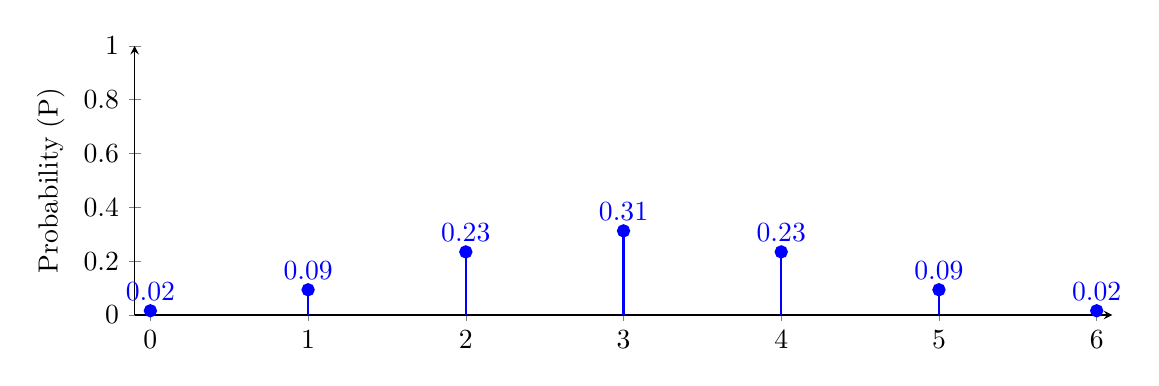
\begin{tikzpicture}
		\pgfkeys{/pgf/number format/fixed}
		\begin{axis}[
			ybar,
			axis lines=left,
			xmin=-0.1, xmax=6.1,
			xtick={0,...,6},
			ylabel={Probability (P)},
			ymin = 0, ymax = 1,
			ytick = {0,0.2,...,1},
			nodes near coords,
			nodes near coords align={vertical},
			width=14cm,height=5cm
			]
		\addplot[ycomb, thick, blue, mark=*] coordinates {(0,0.015625) (1,0.09375) (2,0.234375) (3,0.3125) (4,0.234375) (5,0.09375) (6,0.015625)};
		\end{axis}
		\end{tikzpicture}
	\end{center}
    For $B(6,0.7)$:
    $$E(X) = 6(0.7) = 4.2, \quad \sigma = \sqrt{6(0.7)(0.3)} = \sqrt{1.26} \approx 1.122$$
    \begin{center}
		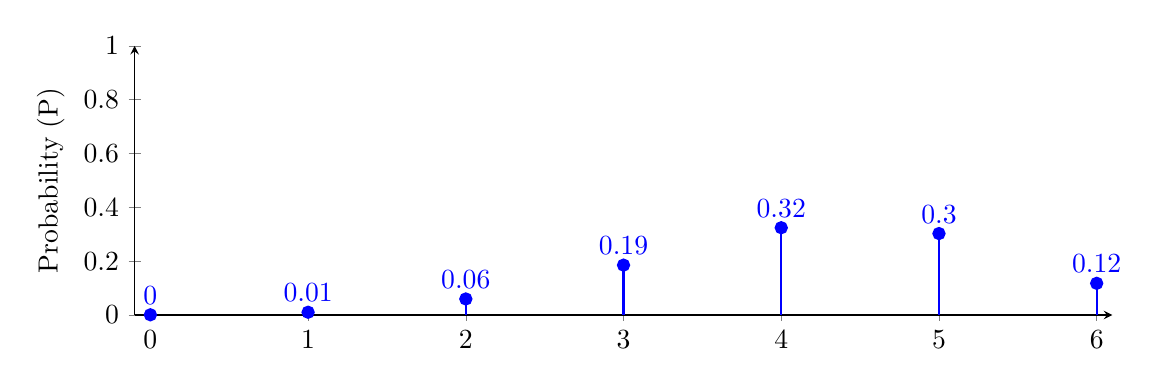
\begin{tikzpicture}
		\pgfkeys{/pgf/number format/fixed}
		\begin{axis}[
			ybar,
			axis lines=left,
			xmin=-0.1, xmax=6.1,
			xtick={0,...,6},
			ylabel={Probability (P)},
			ymin = 0, ymax = 1,
			ytick = {0,0.2,...,1},
			nodes near coords,
			nodes near coords align={vertical},
			width=14cm,height=5cm
			]
		\addplot[ycomb, thick, blue, mark=*] coordinates {(0,0.000729) (1,0.010206) (2,0.059535) (3,0.18522) (4,0.324135) (5,0.302526) (6,0.117649)};
		\end{axis}
		\end{tikzpicture}
	\end{center}
    \item A fair die is rolled 8 times. Calculate the probability that there are:
    \begin{enumerate}
        \item Exactly 5 even numbers
        $$P(X=5) = {8 \choose 5}(0.5)^5(0.5)^3 = {8 \choose 5}(0.5)^8 = 56(0.00390625) = 0.21875$$

        \item Exactly one 6
        $$P(X=1) = {8 \choose 1}(1/6)(5/6)^7 = 8(1/6)(0.27908) \approx 0.3721$$

        \item No 4s
        $$P(X=0) = (5/6)^8 \approx 0.2326$$
    \end{enumerate}

    \item Consider two independent binomial random variables $X_1 \sim B(n_1,p)$ and $X_2 \sim B(n_2,p)$. If $Y = X_1 + X_2$, explain why $Y \sim B(n_1 + n_2, p)$.\\
    Since $X_1 \sim B(n_1,p) \Rightarrow X_1=A_1+A_2+\dots+A_{n_1}$ and $X_2 \sim B(n_2,p)\Rightarrow X_1=A_{n_1+1}+A_{n_1+2}+\dots+B_{n_2}$ where $A_i$ is pair wise independent with parameter $p$. Hence
    $$Y = X_1 + X_2 = \sum_{i=1}^{n_2} A_i \sim B(n_1 + n_2, p)$$

    \item If $X$ has a geometric distribution with parameter $p = 0.7$, calculate
    \begin{enumerate}
        \item $P(X=4)$
        $$P(X=4) = (1-p)^{3}p = (0.3)^3(0.7) = 0.0189$$

        \item $P(X=1)$
        $$P(X=1) = p = 0.7$$

        \item $P(X \le 5)$
        $$P(X \le 5) = 1 - (1-p)^5 = 1 - (0.3)^5 = 1 - 0.00243 = 0.99757$$

        \item $P(X \ge 8)$
        $$P(X \ge 8) = (1-p)^{7} = (0.3)^7 = 0.0002187$$
    \end{enumerate}

    \item Suppose that $X_1, \ldots, X_r$ are independent random variables, each with a geometric distribution with parameter $p$. Explain why
    $$Y = X_1 + \cdots + X_r$$
    has a negative binomial distribution with parameters $p$ and $r$. Use this relationship to establish the mean and variance of a negative binomial distribution.\\
    Negative binomial distribution counts the number of trials until the $r$-th success. Another way to think of this is the trials until the 1st success, and 2nd success, \dots $r$th success with parameter $p$. Hence, 
    $$E(Y)=E(X_1 + \cdots + X_r)=\sum_{i=1}^{r}E(X_i) = \sum_{i=1}^{r}\frac{1}{p}$$
    $$\n{Var}(Y)=\n{Var}(X_1 + \cdots + X_r)=\sum_{i=1}^{r}\n{Var}(X_i)=\sum_{i=1}^{r}\frac{(1-p)}{p^2} = \frac{r(1-p)}{p^2}$$
    \item If $X$ has a negative binomial distribution with parameters $p = 0.6$ and $r = 3$, calculate:
    \begin{enumerate}
        \item $P(X=5)$
        $$P(X=5) = {5-1 \choose 3-1}(0.6)^3(0.4)^{2} = {4 \choose 2}(0.216)(0.16) = 6(0.03456) = 0.20736$$

        \item $P(X=8)$
        $$P(X=8) = {8-1 \choose 3-1}(0.6)^3(0.4)^{5} = {7 \choose 2}(0.216)(0.01024) = 21(0.00221184) = 0.04645$$

        \item $P(X \le 7)$
        $$P(X \le 7) = \sum_{x=3}^{7} {x-1 \choose 2}(0.6)^3(0.4)^{x-3} \approx 0.952$$

        \item $P(X \ge 7)$
        $$P(X \ge 7) = 1 - P(X \le 6) \approx 1 - 0.901 = 0.099$$
    \end{enumerate}

    \item An archer hits a bull's-eye with probability $0.09$ and results of different attempts are independent.
    \begin{enumerate}
        \item Probability that the first bull's-eye is scored with the fourth arrow:
        $$P(X=4) = (1-0.09)^{3}(0.09) = 0.91^{3}(0.09) = 0.0684$$

        \item Probability that the third bull's-eye is scored with the tenth arrow:
        $$P(X=10) = {9 \choose 2}(0.09)^3(0.91)^7 = 36(0.000729)(0.501) = 0.0132$$

        \item Expected number of arrows before first bull's-eye:
        $$E(X) = \frac{1}{p} = \frac{1}{0.09} \approx 11.11$$

        \item Expected number of arrows before third bull's-eye:
        $$E(X) = \frac{r}{p} = \frac{3}{0.09} = 33.33$$
    \end{enumerate}
\end{enumerate}
